\section{8. Medici\'on de se\~nales sinc y tren de pulsos}

\subsection{An\'alisis te\'orico}

\subsubsection{Diagramas espectrales}

\paragraph{Se\~nal sinc:} Se desea encontrar el espectro en frecuencia de la se\~nal sinc, la cual suede denominarse una se\~nal pseudo-peri\'odica
dado el car\'acter repetitivo de la forma de onda, a pesar de que sus valores de amplitud se encuentre en decremento al pasar el tiempo. Utilizando un senoide
de frecuencia $f_o$ se define como en la Ec. \ref{eq:definicion_sinc_ejercicio_8} la se\~nal a transformar.

\begin{equation}
    x(t) = sinc(2 \cdot f \cdot t) = \frac{sin(2 \pi \cdot f_o \cdot t)}{2 \pi \cdot f_o \cdot t}
    \label{eq:definicion_sinc_ejercicio_8}
\end{equation}

Entonces, por definici\'on llamando $\tau = 2 \cdot f$, se puede encontrar su transformada de Fourier, y resulta en la expresi\'on
hallada en la Ec. \ref{eq:transformada_sinc_ejercicio_8}.

\begin{equation}
    F \left[ x(t) \right](f) = \frac{1}{2 \cdot f_o} \cdot \Pi \left( \frac{f}{2 \cdot f_o} \right)
    \label{eq:transformada_sinc_ejercicio_8}
\end{equation}

\begin{figure}[H]
    \centering
    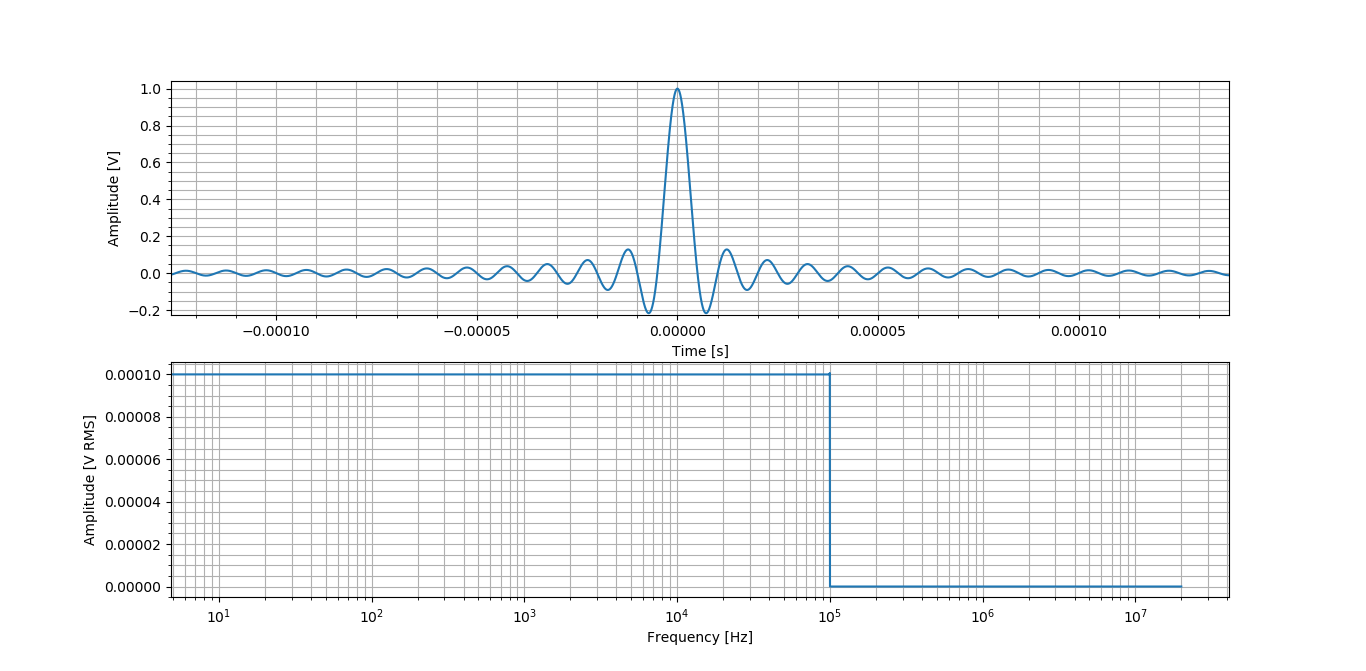
\includegraphics[scale=0.45]{Recursos/sinc.png}
    \caption{Diagrama espectral en magnitud de funci\'on Sinc}
\end{figure}

\paragraph{Se\~nal tren de deltas de Dirac:} En este caso se define la se\~nal de la forma en la cual se muestra en la Ec. \ref{eq:definicion_deltas_dirac_ejercicio_8} y luego
se la transforma a Fourier, obteniendo el resultado de la Ec. \ref{eq:transformada_deltas_dirac_ejercicio_8}.

\begin{equation}
    x(t) = \sum_{n = - \infty}^{\infty} \delta(t - \frac{n}{f_o})
    \label{eq:definicion_deltas_dirac_ejercicio_8}
\end{equation}

\begin{equation}
    X(f) = F \left[ x(f) \right](f) = \frac{1}{T} \cdot \sum_{n = - \infty}^{\infty} \delta(f - n \cdot f_o)
    \label{eq:transformada_deltas_dirac_ejercicio_8}
\end{equation}

\begin{figure}[H]
    \centering
    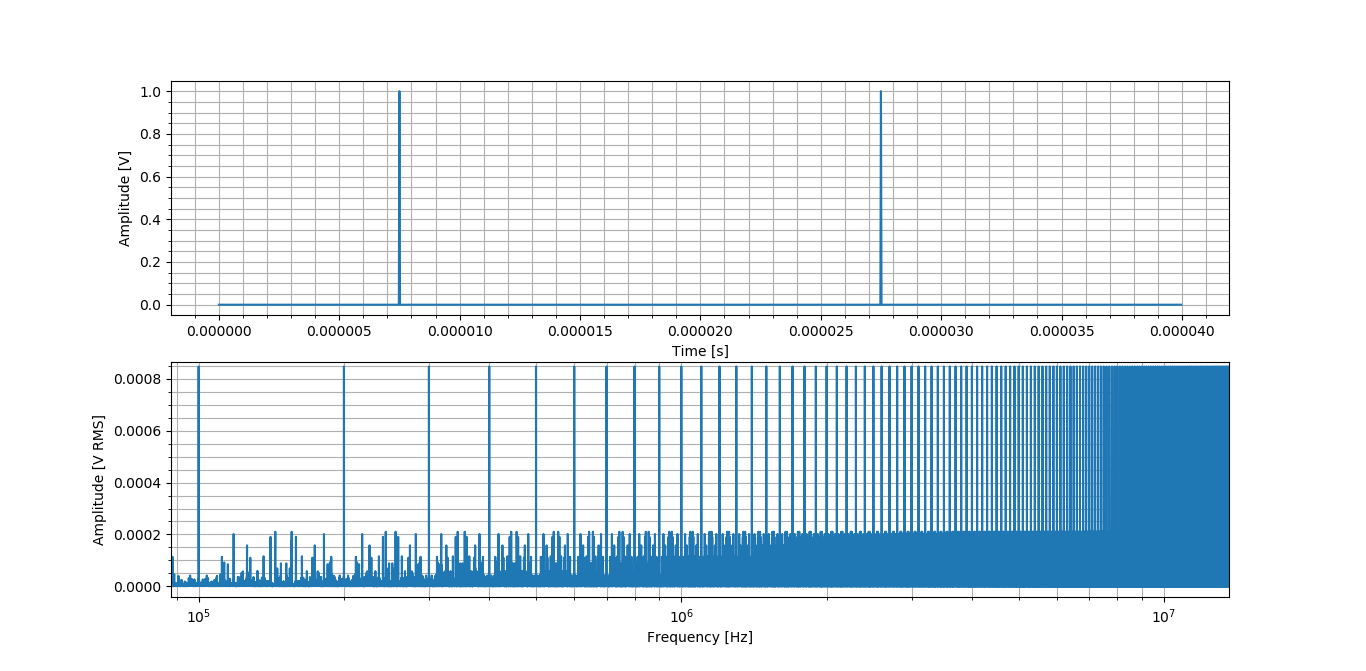
\includegraphics[scale=0.45]{Recursos/tren_delta_dirac.png}
    \caption{Diagrama espectral en magnitud del tren de deltas}
\end{figure}

Como puede observarse, ambas se\~nales tienen un contenido espectral que no es finito, pero a pesar de ello se distinguen una de otra
por el hecho de que para el caso del tren de deltas de Dirac, sus arm\'onicos est\'an discretizados, mientras que no sucede as\'i con el caso de 
la se\~nal sinc, cuyo espectro es continuo.

\subsection{Mediciones}

\begin{figure}[H]
    \centering
    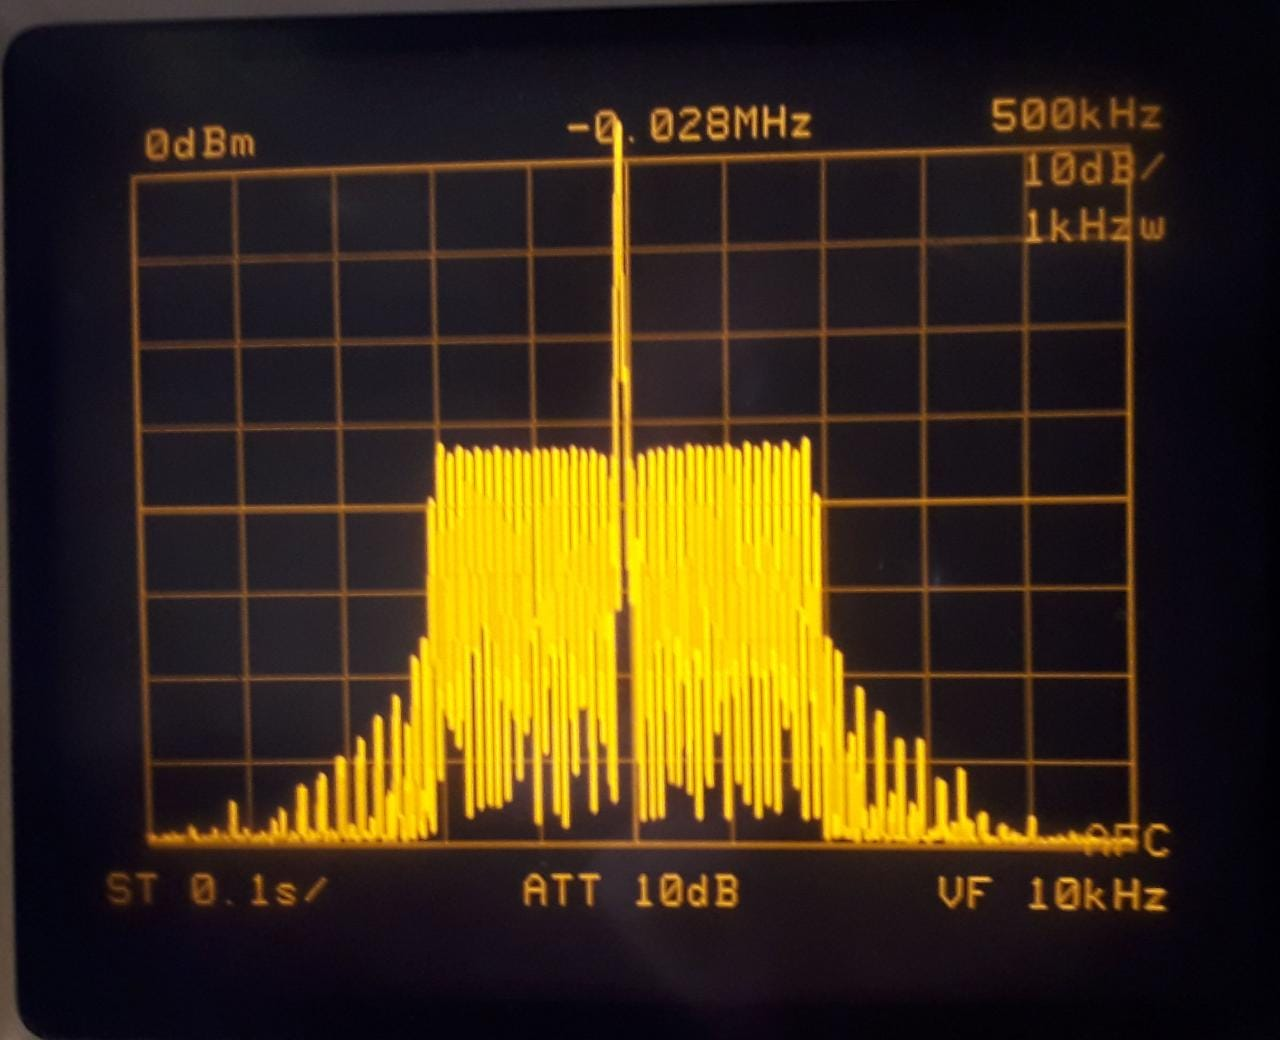
\includegraphics[scale=0.2]{../Mediciones/Ejercicio_8/ej8_espectro_sinc.jpeg}
    \caption{Espectro de la se\~nal sinc}
    \label{fig:ej8_espectro_sinc}
\end{figure}

\begin{figure}[H]
    \centering
    \begin{tabular}{c c}
        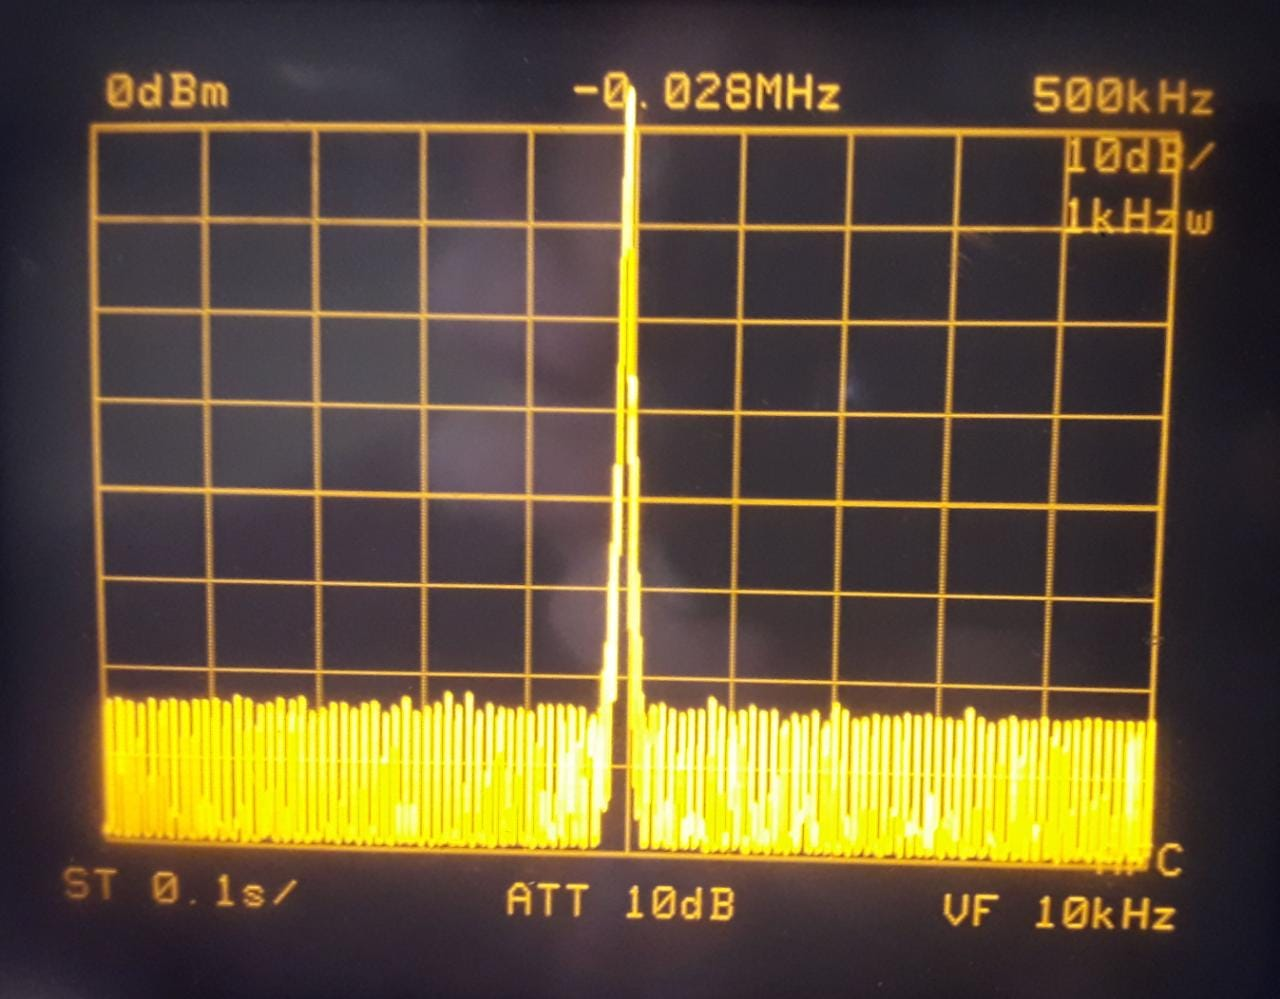
\includegraphics[scale=0.185]{../Mediciones/Ejercicio_8/ej8_espectro_deltas.jpeg} &
        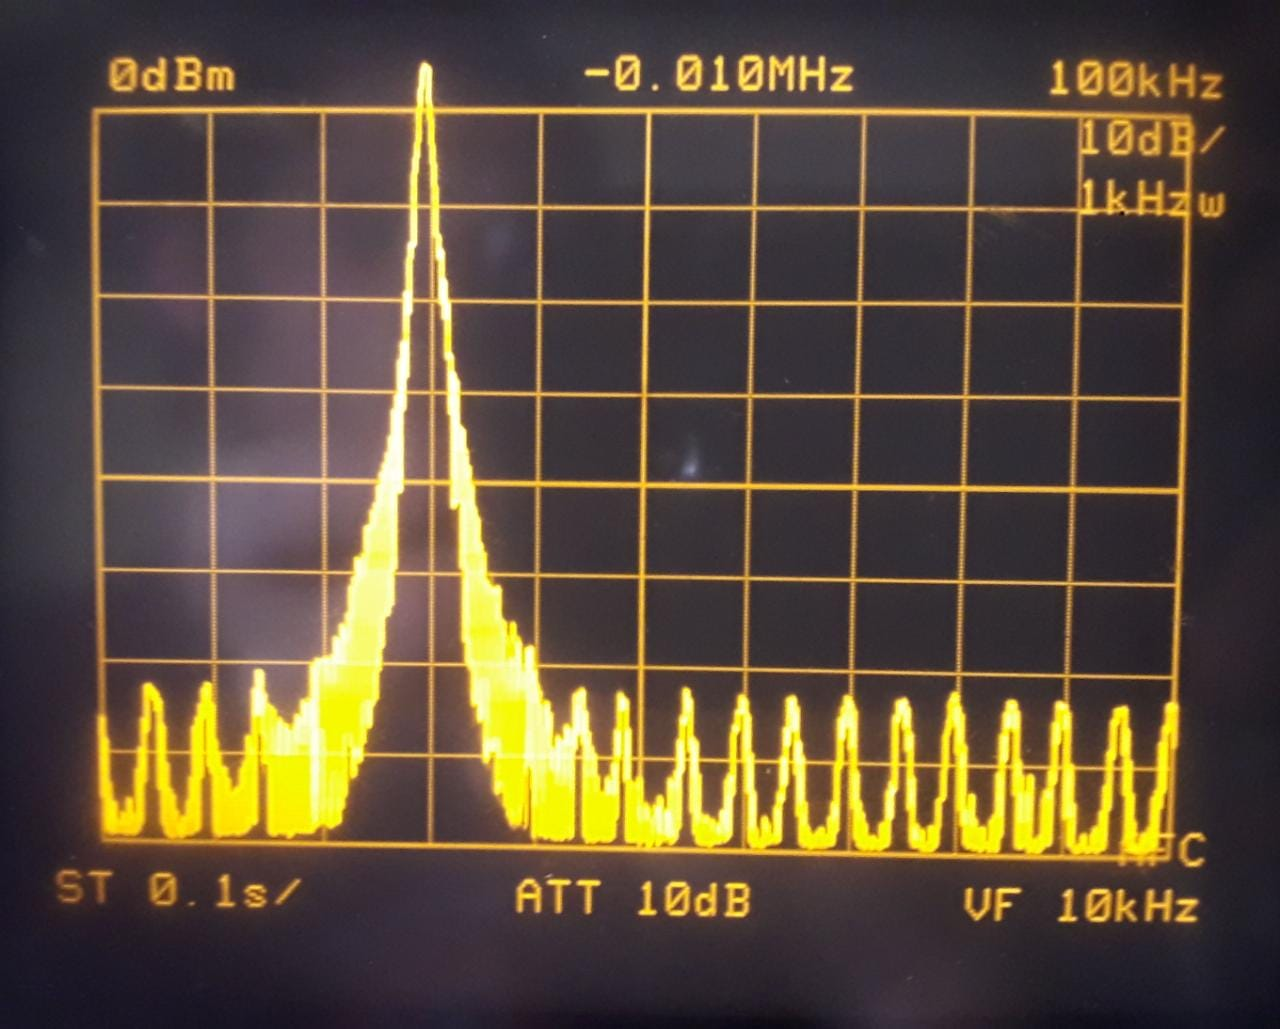
\includegraphics[scale=0.18]{../Mediciones/Ejercicio_8/ej8_espectro_deltas_zoom.jpeg}
    \end{tabular}
    \caption{Espectro de la se\~nal tren de deltas}
    \label{fig:ej8_espectro_deltas}
\end{figure}

\subsection{An\'alisis de los resultados}
Se pudo observar y corroborar el espectro esperado como resultado para ambas ondas,
donde en primer lugar el espectro resultante de la onda $\frac{sin(x)}{x}$ deber\'ia ser un pulso,
pero se asume que por caracter\'isticas del barrido en el oscilador local del analizador, las muestras producen sucesivos deltas
que hacen a la forma de un pulso. Se llega a la conclusi\'on de que los arm\'onicos que aparecen luego del pulso son desperfectos
ya sea por alguna distorsi\'on arm\'onica del generador, o bien resultado de la medici\'n del analizador.

Finalmente, en las Fig. \ref{fig:ej8_espectro_deltas} se pueden ver las infinitas componentes del tren de deltas, con una amplitud
peque\~na.
